\documentclass[conference]{IEEEtran}
\IEEEoverridecommandlockouts
\usepackage{cite}
\usepackage[hyphens,spaces,obeyspaces]{url}
\usepackage{amsmath,amssymb,amsfonts}
\usepackage{algorithmic}
\usepackage{graphicx}
\usepackage{textcomp}
\usepackage{xcolor}
\usepackage{csquotes}
\usepackage{listings}
\def\BibTeX{{\rm B\kern-.05em{\sc i\kern-.025em b}\kern-.08em
    T\kern-.1667em\lower.7ex\hbox{E}\kern-.125emX}}
\begin{document}

\title{A Strategy Video-Game for Collaborative Agents with a Personality and Humoristic Dialogues\\
}

\author{\IEEEauthorblockN{Jordan Mackie}
\IEEEauthorblockA{\textit{Student}}
\and
\IEEEauthorblockN{Alice Toniolo}
\IEEEauthorblockA{\textit{Supervisor}}
\and
\IEEEauthorblockN{Christopher Stone}
\IEEEauthorblockA{\textit{Supervisor}}
}

\maketitle

\begin{abstract}

	We built a system of collaborative agents with personality driven decisions and humoristic dialogues with the goal of providing entertainment and also providing a human friendly way of interpreting agent interactions in multiagent systems. The agents were designed to play chess and given goal-based personalities that would affect their decisions and how they would interact with other agents. We gathered feedback through allowing volunteers to play against our agents and asking questions covering usability and enjoyment. Finally, we present our results and discuss further work or areas of improvement that could be taken up.

\end{abstract}

\section{Introduction}

Multiagent systems are the next step to increase the level of autonomy that can be provided by technology. Agents that are able to learn, adapt, and negotiate with other agents to achieve their goals allow for complex problems to be solved or modelled without human intervention, such as monitoring and maintaining national power grids \cite{archon}. 

Often, developers and users will anthropomorphise these agents when describing their behaviour. This project aims to encourage this by implementing agents with a model of personality that affects their choice of actions, by rendering the negotiations between agents in a natural language, and by using models of humour to make the interactions between agents entertaining. 

Chess was chosen as our strategy game as multiagent implementations have been previously investigated, though not in a configuration where agents could have conflicting goals in the same team. However, our model for determining agent actions can be applied to any other strategy game or multiagent system.

\section{Context Survey}

\subsection{Multiagent Systems in Entertainment}

Many modern video games involve the user managing multiple characters to achieve some goal, such as producing in-game resources or defending against an opponent. This sort of problem lends itself easily to multiagent systems. Instead of having one artificial intelligence engine driving the actions of all the characters, developers can create agents with a limited set of actions and some concept of progress towards their goals and allow emergent behaviour to find a solution to the problem, sometimes in surprising ways. 

\cite{sandboxmas} discuss how multiagent systems can be applied to create more realistic worlds in sandbox games. By implementing the environment, objects, and non-playable characters (NPCs) as agents, developers can create a world that reacts and adapts the player, but also operates in isolation from the character to provide a realistic setting. The concept of personalities is also mentioned as a way of allowing similar NPCs to exhibit different slightly different behaviours, such as having aggressive or relaxed driving styles.

Even in games with very simple rules and logic, multiagent systems can find interesting and complex solutions. OpenAI implemented hide-and-seek using agents, where hiders avoid the line-of-sight of the seekers \cite{openaiemergent}. The game was played in a world with randomly generated walls and objects such as ramps (for climbing over walls) and blocks (for forming barricades). What made this fascinating is that the agents were not incentivised to use these objects, but after repeatedly playing and learning, both the hiders and seekers created strategies such as blocking each other in a safe area, and even removing the objects from the other team before hiding.

Knowing that multi-agent autocurricula can realise strategies not considered by humans, \cite{masboardgames} discuss how they can be applied to strategy board games such as Diplomacy and Risk. They describe a generic framework for supporting agent-based competitive bots for board games and then implement bots for the aforementioned games. Their research suggests that for games with a large number of units and a large action space, a multi-agent approach can identify effective strategies quicker than the exhaustive methods used for chess engines. 

\subsection{Multiagent System Frameworks}

Most multiagent systems have similar requirements, and so several frameworks have been developed to bootstrap their development. \cite{massurvey} provide a very thorough survey of the frameworks currently in use today and highlight various features and drawbacks in their implementation. 

The most popular is the Java Agent Development Framework (JADE) \cite{jade}. It conforms to the FIPA standard, which is a protocol for agent communication that involves defining performatives (e.g. request, inform), language name, and other message meta-data during communication. The benefit of systems that abide this standard is that they are able to interact regardless of the technology used to implement them. JADE provides other important features such as base classes for agent functionality called behaviours, a directory facilitator (DF) agent implementation to allow agents to find each other, and an Agent Management Service that manages and tracks the lifecycle of agents and allows them to move between containers (which can exist on multiple hosts). To aid during development, JADE also incldues a GUI for debugging and manually interacting with agents.

Other frameworks provide APIs that encourage certain design patterns. For example, Jason was built to support the belief-desire-intention (BDI) design model which attempts to seperate the processing of choosing a plan from the execution of the chosen plan \cite{jason}. Jason provides many of the same functionalities as JADE, but the latter was chosen due to being slightly more flexible.

\subsection{Models of Personality and Emotion}

Creating a truly immersive video game requires characters that the player can empathise with. Robots have been shown to be able to influence human behaviour as an authority figure \cite{bossrobot} and when begging not to be turned off \cite{turnoffrobot} by expressing emotions. \cite{personalitymodel} created and demonstrated a model of personality and emotion that would allow agents to react differently to the same stimulation. For example, when a agent with an 'introverted' personality is offered help, they are less likely to accept it due to the prolonged interaction it would entail. 

\cite{skyrim} also created a model that would use personality, emotion, and social relationships to determine the behaviour of NPCs in a video game. The frequency and tone of interactions between NPCs as well as the NPC and the player were accounted for when choosing facial expressions and tone of voice during conversations. Test subjects described feeling especially attached to the NPCs that utilised this model.

A useful aspect of multiagent systems is that agents can be developed in isolation but still interact (e.g. an agent that searches for cheap transport options and an agent responsible for auctioning train tickets could be developed separately with no knowledge of the logic being used by the other). \cite{hetrogenousagents} discuss how developing heterogeneous agent systems using personalities and social structures could help when dealing with third-party agents that have been constructed to lie and exhibit selfish or uncooperative behaviour.

\subsection{Collaborative Argumentation}

Knowledge is distributed in a multiagent system therefore specialist agents need to be able to alter the beliefs of others by appealing to their individual goals. \cite{argumentation} implemented a framework that achieves this based on a scheme given by \cite{reasoning}:

\begin{displayquote}
	In the current circumstance R, we should perform action A, which will result in new circumstances S, which will realise goal G, which will promote some value V.
\end{displayquote}

Specifically, they were able to create a framework for multiple parties to discuss and collaborate which could greatly affect the design of multiagent systems that utilise it. By producing an ontology which any agents involved in the discussion understand, goals and circumstances can be conveyed through the use of predicates and concepts. Conveniently, JADE already provides an API for creating ontologies. However, the manual work required to construct an ontology that captures the components and logic of a game of chess was found to be far too cumbersome. While this would be the most interoperable solution, serializable Java objects were used instead for quicker development. 

The overhead of argumentation required in multiagent systems can be a quick filter to determine which problems it is a suitable solution for. For example, \cite{argumentationcontext} investigated how quickly agents that used collaborative argumentation to achieve global consistency in a time-constrained task (i.e. escaping a burning building) performed. Their results suggest that optimisations or different approaches to the protocol design would likely be necessary for a real-time strategy game, but it could depend on many factors such as the number of agents, the distribution of knowledge, and more.

Previous work has shown that multiagent chess systems do not generally perform well strategically compared to normal tree based models for chess if the agents are given any limitations that restricts their knowledge. \cite{agentchess} limited pieces such that they could only evaluate their immediate surroundings, and all pieces would reach a consensus based which focused on maximising captures and minimising losses. Our solution will not limit the agents knowledge of the board, but pieces will still have to reach some consensus on which move to take based on their own individual values. 

\subsection{Natural Language Generation}

In order to make the discussions between agents more entertaining and user-friendly to observe, our project involves using natural language generation (NLG) methods to translate the messages or agent intent to plain English. \cite{owlnlg} built an NLG system for a particular ontology language (W3C Ontology Language a.k.a. OWL), which is able to construct texts corresponding to objects and their properties in the ontology in English and Greek. \cite{rdfnlg} achieved similar results for one of the other Semantic Web Formalisms (specifically RDF) and were able to produce instructions for cooking recipes from a corpus of data in a far less human-friendly format. They were even able to adjust the level of technical jargon in the resulting text to accommodate for the readers familiarity with cooking. The ontology allowed for optimised searching of the parse trees but they also required a domain corpus (i.e. existing textual recipes) in order to properly train their natural language generator. Their solutions are specific to the Semantic Web project, and would not produce "conversations" like we are planning to do, but provide a good foundation for implementing this functionality.

Generic frameworks have also been created that are not based strictly on ontologies which were also considered. For example, SimpleNLG \cite{simplenlg} is an NLG engine that allows for valid English phrases to be constructed through a very simple Java API. However, after some time experimenting with this library, it was realised that it was very difficult to reliably produce a variety of phrases, though it was useful for controlling features such as grammatical person and tense.

\cite{robotgame} created a robot capable of providing dialogue while playing against a human at tic-tac-toe, but used a slot-filling technique based on templates that suffered from little flexibility and left no room for personality in dialogue creation. Contrarily, systems such as Siri and Alexa are examples of successful dialogue systems that have been able to provide assistance to humans in the form of natural language conversations by avoiding the template based approaches.

These systems instead take advantage of machine learning techniques such as deep recurrent neural networks (DRNN). \cite{dialoguesystems} surveyed projects that applied these modern techniques for NLG, and concluded that in order to account for aspects such as current state of the program during the execution of conversation as our project requires, a hybrid of the machine learning and rule based approaches may be necessary. 

The dynamic finite-state machine implementation of a chatbot called Tartan \cite{tartan} was also especially useful for the project, as it focused on natural conversation flows rather than the extraction of information from a human user like most other chatbot research. Their conversation state machine design was combined with the RiTa library's RiGrammar (a probabilistic context free grammar) in order to produce a variety of phrases and conversation flows. 

\subsection{Computational Humour}

Simply reading the discussion between agents would certainly not make for an entertaining game, and so adjusting the dialogue or agent behaviour is required. However, artificial humour also has benefits for everyday computing: a smartphone that is able to sympathise with the user when it is unable to connect to a weak WiFi network or cheer them up with a joke when they miss their bus is one that the user is more likely to enjoy using. 

Unfortunately, given humour is an incredibly contextual and culture driven concept, it is no surprise that computational humour is well researched yet still not 'solved'. Jason Rutter describes why using artificial intelligence for humour is particularly challenging:

\begin{displayquote}
"Humour is a very interesting way to look at artificial intelligence because at some point something has to have two meanings, which is not easy to do with a computer." \cite{jasonrutter}
\end{displayquote}

There are three main theories of humour that are used for computational humour: superiority theory (laugh about the misfortune of others), relief theory (using taboo subjects to release tension), and incongruity theory (using lexical and structural ambiguity). The last theory is currently the most popular, and was used during the development of JAPE \cite{jape}. JAPE identifies features such as homophones to produce jokes like:

\begin{displayquote}
	"What is the difference between leaves and a car? One you brush and rake, the other you rush and brake."
\end{displayquote}

However, JAPE does not allow for much user interaction, and most textual humour generation takes the form of simple puns and riddles. Our agents could instead generate situational humour by surprising the user by diverting suddenly from expected behaviour. The Suslov Model of humour accounts for the fact that we subconsciously predict expected conclusions to situations and phrases, and that contradictions in what is the most likely direction for a conversation or situation to what was previously predicted can create a humour response \cite{suslov}.

These probabilistic models currently appear more hopeful than the rule based models used by older implementations such as JAPE. Instead, \cite{humourrnn} used an existing corpus of jokes and a recurrent neural network to produce a system capable of generating jokes and even anti-jokes (jokes without an actual punchline). 

%TODO how did our system achieve the funny?

\section{System Design}

An existing multiagent development framework was chosen instead of rolling our own in order to abstract away matters such as message delivery and agent life-cycle management. As mentioned earlier, JADE was chosen specifically due to its flexibility and its extensive coverage of the FIPA standard that could allow our agents to interact with other implementations with ease. 

With the intention of possibly serving the game over the internet once complete, the system had to be designed to allow for communication with agents from outside of the agent platform. The 'JadeGateway' API was used with a Spring Boot server and React UI to to achieve this. Figure \ref{fig:highlevelarchitecture} provides a high level overview of the technologies at each layer.

\begin{figure}[h]
	\centering
	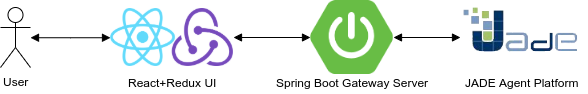
\includegraphics[width=\linewidth]{images/highlevelarchitecture}
	\caption{Technologies used at each layer.}
	\label{fig:highlevelarchitecture}
\end{figure}

\subsection{Front-End}

React \cite{reactjs} was chosen due to it being the most familiar web framework for the developer of this project, and because a component already existed for rendering chessboards \cite{chessboardjsx}. React uses a virtual DOM in order to efficiently re-render components based on changes in state. For example, when a new message arrives, the state of the chat transcript component is updated to contain the new message which triggers an update to only the chat transcript and its children that are also affected. 

As the project grew, Redux \cite{redux} was introduced in order to help with state management of components. Redux provides a single global state which components 'connect' to in order to receive updates. Updates are 'dispatched' as actions, which are then passed through a pipeline of reducers which update parts of the global state depending on the action and its payload. Middleware can also be introduced to allow certain actions to create chains of updates (e.g. making an asynchronously API call, then dispatching another action when the response is received), but the reducers themselves are always pure functions. This functional approach to managing components made the project easier to test and errors easier to trace and correct. Figure \ref{fig:reducers} shows the parts of the state that are managed by each reducer.

\begin{figure}[!h]
	\centering
	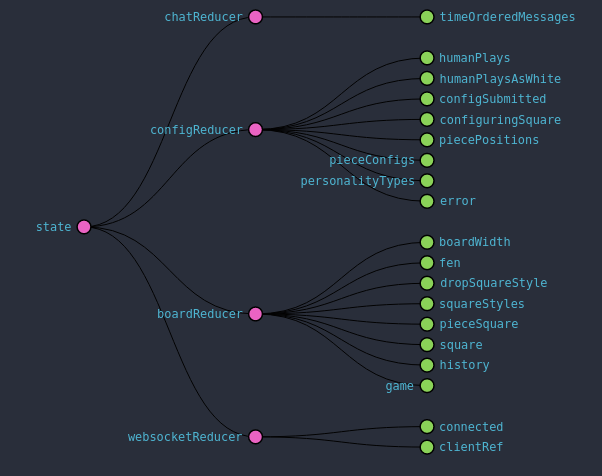
\includegraphics[width=\linewidth]{images/reducers}
	\caption{Redux reducer tree showing which parts of the state are managed by which reducers.}
	\label{fig:reducers}
\end{figure}

One of the challenges faced were that the abstraction of the chessboard component provided by a third-party library did not allow for atypical visual elements such as adding name tags to each piece or dialogue boxes. This then required manually implementing an overlay that would draw another chessboard grid, track positions of pieces, and draw the name tags and dialogue boxes in the correct locations. 

The UI is composed of two main views: configuration and gameplay. 
The configuration view (Figure \ref{fig:configview}) allows the user to choose if they want to play against the agents or watch two sets of agents play against each other. By clicking on the pieces they will not be controlling, the user can also name the pieces and define their personality type. 

\begin{figure}[!h]
	\centering
	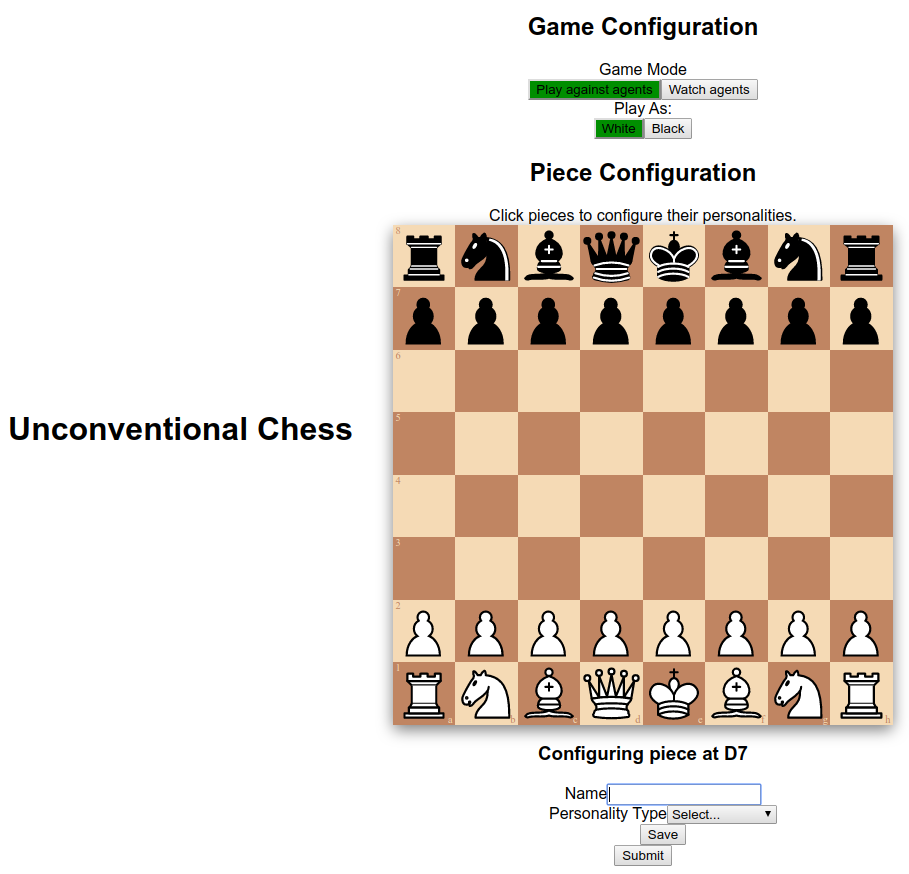
\includegraphics[width=\linewidth]{images/configview}
	\caption{Configuration view.}
	\label{fig:configview}
\end{figure}

On submit, any unconfigured pieces are filled out at random from the set of available personalities and a set of names. The game configuration is then sent as a POST request to the gateway server, which verifies and creates the resources necessary for the game and returns its ID to allow the client to publish and subscribe to game events at the correct web socket endpoint.

Figure \ref{fig:gamecreation} shows the sequence diagram for how resources are created once the user submits the game configuration

\begin{figure}[!h]
	\centering
	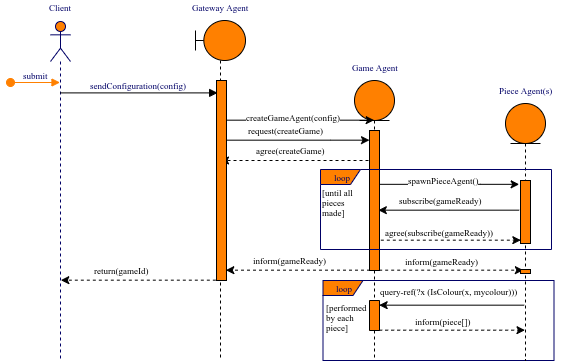
\includegraphics[width=\linewidth]{images/gamecreation}
	\caption{Game creation sequence diagram.}
	\label{fig:gamecreation}
\end{figure}

The game view (Figure \ref{fig:gameview}) also shows the game board with name tags over the corresponding pieces and any dialogue next to the speaking piece. The chat and move history is also rendered in a scrolling transcript at the bottom of the page in alternating colours for clarity. When hovering over pieces the user is able to see all currently available moves to them. Moves are verified client side by the chess.js \cite{chessjs} engine before either being rejected or sent to the server. Figure \ref{fig:humanmove} shows how human moves are broadcast to all subscribers.

\begin{figure}[!h]
	\centering
	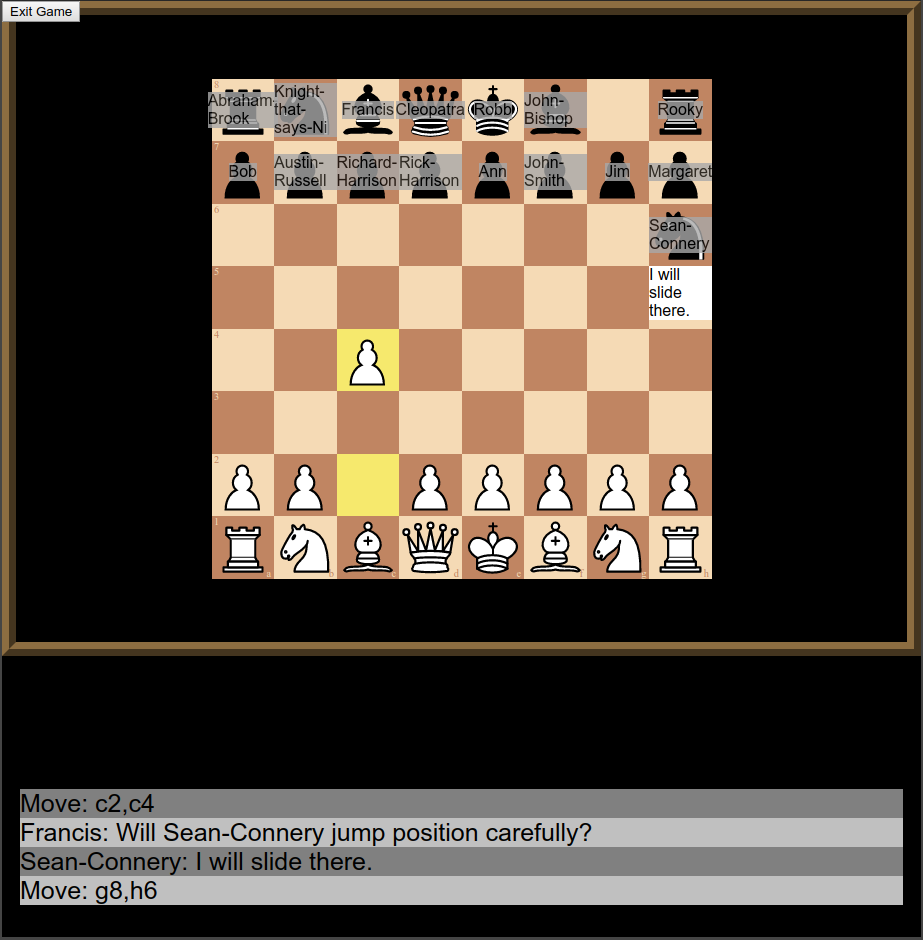
\includegraphics[width=\linewidth]{images/gameview}
	\caption{Game view.}
	\label{fig:gameview}
\end{figure}

\begin{figure}[!h]
	\centering
	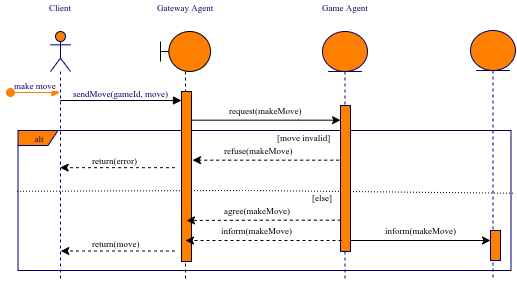
\includegraphics[width=\linewidth]{images/humanmove}
	\caption{Human move sequence diagram.}
	\label{fig:humanmove}
\end{figure}

\subsection{Agent Gateway Server}

The gateway server has several purposes: 
\begin{itemize}
	\item{Serve the web app}
	\item{Handle game resources}
	\item{Route messages between users and relevant agents}
\end{itemize}

JADE does have support for agents serving web resources directly, but the JadeGateway API was used instead as it was simpler to set up. The JadeGateway API effectively creates an Agent for the server, which can then send units of functionality called 'Behaviours' to be executed by the agent (e.g. sending messages to the agents within the platform). This could potentially be a bottleneck if the number of users of the server was to grow large enough due to agents being single-threaded by default, so an implementation at scale would likely need to change this interface. For the purposes of this project however, it was more than sufficient.

On start-up, the server uses the details in a configuration file to connect to the JADE platform. It also exposes a limited set of HTTP endpoints to allow the client to create games and to query available personality types. An in-memory message broker is used for handling websocket sessions once a game is set up so that clients can subscribe to chat and move messages, and send their own moves. 

The JadeGateway polls for incoming messages using the \lstinline{ListenForGameAgentMessages} behaviour, which is provided a message translator and a message handler for translating \lstinline{ACLMessage}s from agents to a data model the server can work with and passing the message to the correct handler. This behaviour allowed the server to utilise JADEs scheduling system which would only run the behaviour if a new message was received, instead of busy waiting for incoming messages.

\subsection{Jade Agent Platform}

Finally, the agent platform is where all of the agents are hosted. Here we will give a rough overview of how JADE agents schedule their functions, while in section \ref{sec:agentimpl} we discuss the actual logic that drives our agents.

JADE agents are single-threaded by default, and execute behaviours according to the flow diagram shown in Figure \ref{fig:behaviour}. The basic JADE behaviour implements the methods shown in figure \ref{fig:behaviour}, but the framework also provides some helper implementations such as the \lstinline{FSABehaviour} which was used heavily during this project. 

Behaviours are scheduled such that they are executed repeatedly round-robin until either they are complete (\lstinline{done()} returns true) or \lstinline{block()} is called during the \lstinline{action()} method. The latter puts the behaviour into a waiting queue so that it is only triggered again once the agent receives a message. 

Behaviours can filter the messages that are received using the \lstinline{MessageTemplate} class, which uses pattern matching to only allow for messages containing features such as a specific performative (e.g. REQUEST, PROPOSE) or a specific conversation ID. This ensures that behaviours do not consume messages that were not intended be consumed by them. 

\begin{figure}[!h]
	\centering
	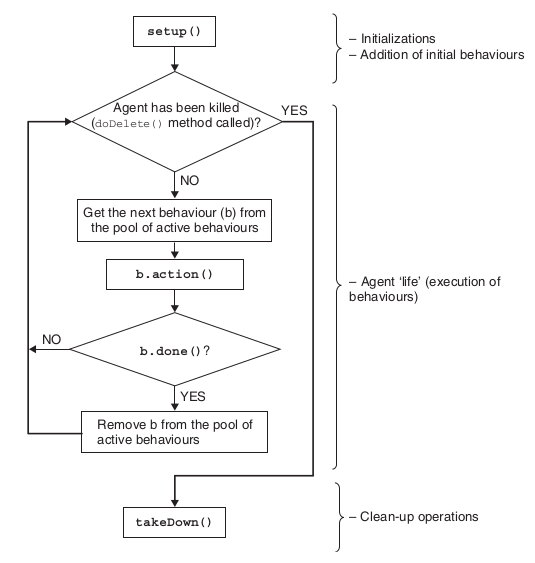
\includegraphics[width=\linewidth]{images/behaviour}
	\caption{JADE Agent behaviour scheduling and life-cycle \cite{jade}.}
	\label{fig:behaviour}
\end{figure}

\section{Agent Implementation} \label{sec:agentimpl}

Our implementation involves two different types of agent: game agents and piece agents. Game agents are responsible for maintaining the state of the game and initialising the piece agents, and piece agents represent pieces on the board, each trying to achieve their own individual goals.

\subsection{Game Agent}

The game agent upon creation waits for a request to begin a chess game. It also answers any queries regarding the current status of the game and information about the pieces being represented by agents. The FIPA standard protocols for agent interaction \cite{fipaprotocols} were followed so that the game agent could provide a consistent API for any implementation of piece agents. For example, the request interaction is used for triggering moves as shown in figure \ref{fig:humanmove}. 

Requests for information are semantic logic expressions with variables which the game agent then populates in its reply. For example, agents wishing to receive updates whenever a new move is made will send a message with a SUBSCRIBE performative and the expression:

\begin{equation} \label{eq:movesubscribe}
	(\;iota\; ?Move\; ("Move Made"\; ?Move))	
\end{equation}

This will then be replied to every time a new move occurs with the variables given values, for example when a piece moves from B8 to C6:

\begin{multline} \label{eq:movesubscribe}
	((=\; (iota\; ?Move\; ("Move Made"\; ?Move))\;  \\
	(Move\; :Source\; (Position\; :Coordinates\; B8)\; \\
	:Target\; (Position\; :Coordinates\; C6))))
\end{multline}

Once the game has started, the game agent adheres to the FSA shown in figure \ref{fig:gameagentfsa}. 

\begin{figure}[!h]
	\centering
	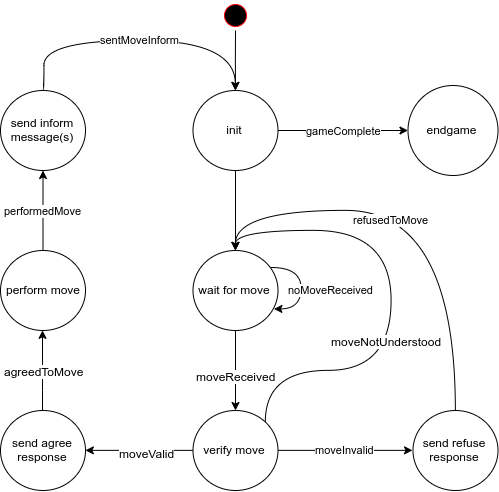
\includegraphics[width=\linewidth]{images/gameagentfsa}
	\caption{Game Agent game handling FSA.}
	\label{fig:gameagentfsa}
\end{figure}

The actual chess logic is managed by a third party library \cite{chesslib}. While this saved a lot of time by providing a way of quickly validating moves, generating valid moves, and tracking the board state, it suffered from the same problem as the chessboard component used by the front-end: it did not provide a way to differentiate between each piece of the same type. This resulted in a wrapper class being implemented which would maintain the mapping between the set of our custom piece representation and the third party board pieces. In hindsight it was clear that it would have been simpler to have implemented the chess logic ourselves, but the wrapper solution was sufficient.

\subsection{Piece Agent}

The piece agent implementation is the focus of this project. They are initialised with their piece type, colour, personality type, and starting position on the board. They are notified by the game agent once the game is ready and whenever a move is made successfully either by the human or another agent. 

\subsubsection{Game State}

The GameState class wraps our chessboard wrapper to provide another layer of abstraction in order for the state of the board to be an immutable object. This was done to avoid complicated undo logic when agents wanted to 'test' moves and evaluate the board after a move is made. Instead, when the \lstinline{applyMove(PieceMove move)} function is called, a copy of the board is made. This involved copying the set of alive and captured pieces, as well as updating the piece objects themselves if any changed position. 

In order to reduce the amount of objects being created and destroyed by this process, piece instances would only be copied if they had changed state in some way (captured/changed position). 

\subsubsection{Personalities and Reasoning}

Agent personalities were designed based on the goal-based trait/value model defined by \cite{hetrogenousagents}. Figure \ref{fig:personalityuml} shows the UML class diagram for our implementation. The personality is initialised with a set of traits (e.g. shy, aggressive) which each have a set of values. Values define what the agent will interpret as good and bad moves based on some criteria (avoid other pieces, maxmise captures). The value class is abstract and is extended by implementations that when given a witnessing piece, the current game state, and a move, are able to produce a response to that move.

\begin{figure}[!h]
	\centering
	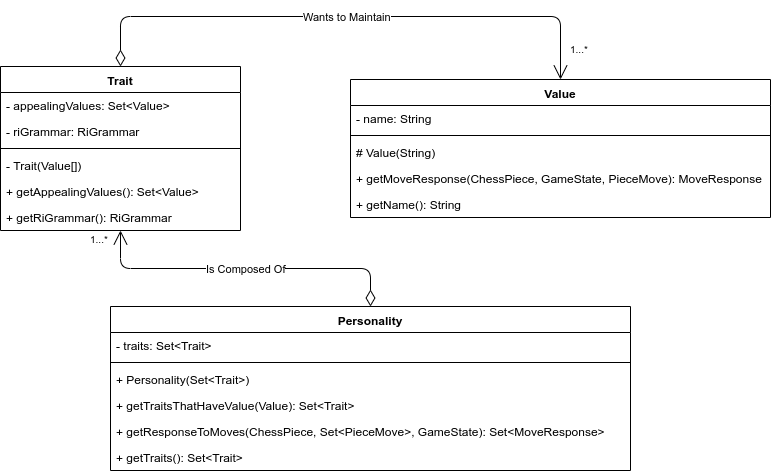
\includegraphics[width=\linewidth]{images/personality}
	\caption{UML Diagram of Agent Personalities.}
	\label{fig:personalityuml}
\end{figure}

This implementation allows different traits to share goals. The move most preferred by an agent is the one that appeals to the most of it values, and so consensus can be reached by finding the move that appeals to the most pieces, even if they have different values.

\subsubsection{Single Thread of Conversation Protocol}

In order to make the conversation between agents seem natural and remain easy to follow, a protocol had to be established to ensure that one agent would speak at a time. The project was initially constructed with conversation flow dictated strictly by a finite state machine. This solution was incredibly restrictive as it required providing a transition path for any conversation path that we wanted to support. After reviewing the work by \cite{tartan} and finding that this strict FSA approach was inherently detrimental to producing natural conversation flows, the original design was thrown out and replaced with the simpler and far more flexible model shown in Figure \ref{fig:conversationfsa}.

\begin{figure}[!h]
	\centering
	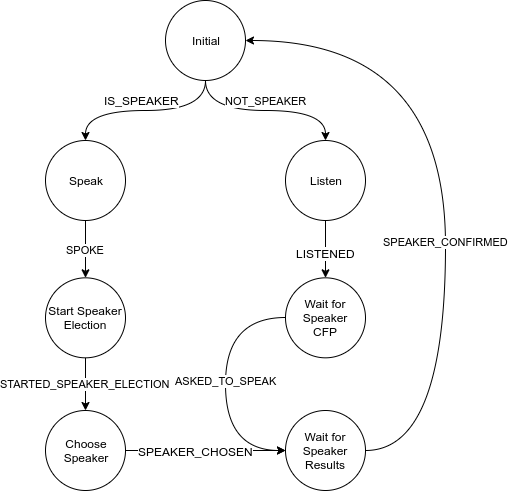
\includegraphics[width=\linewidth]{images/conversationfsa}
	\caption{Conversation protocol FSA}
	\label{fig:conversationfsa}
\end{figure}

The conversation FSA designed by \cite{tartan} was for a human-agent chatbot, and so was adapted to include a token-passing protocol to determine which agent would speak next. One of the benefits of this design is that it allowed for the agents to chat throughout the game, not just during their turn. This meant that the agents could provide ambient conversations and respond to events like the previously made move while the human player chose their next move.

At the start of each turn (i.e. when a new move is received or the very first turn of the game), each agent returns to the initial state to ensure that they are all synchronised. The king is assumed first to speak. The other pieces listen for any messages from the speaker and the speaker chooses what to say. Once sent, the speaker begins the new speaker election by sending a call for proposal (CFP) message to all alive pieces (and themselves), and waits until every pieces has submitted a proposal to be the next speaker. Finally the speaker chooses from the set of proposals, sends a rejection to all but the chosen speaker, and then the cycle begins anew.

The requirement that all agents reset to the initial state at the start of each turn was necessary to avoid race conditions during the speaker election. For example, if a move was received that resulted in one of the agents being captured, that agent would immediately remove themselves from the game. However, if that agent was the speaker during an election, then all other agents would be stuck waiting for the next speaker to be chosen. Whilst other solutions would allow for the conversation flow to continue, it was deemed much simpler to reset the conversation FSA during each turn.

As a side effect of this decision, messages such as the speaker election CFP could be waiting an agents message queue if they reset before receiving it. To avoid this resulting in a loss of synchronisation between agents, a new conversation ID is assigned during each cycle of the FSM which is composed of the turn ID (i.e. how many moves have been made so far) and the round ID (how many cycles of the conversation FSA have occurred this turn). The conversation ID is used to filter incoming messages to ensure that irrelevant messages are ignored. Unfortunately this could result in a build-up of expired messages over time, but given most chess games were around 80 moves \cite{chessdata} and roughly 5 messages per move would be lost in the queue, the leak would not be substantial. Especially when we considered that the messages would be garbage collected once the agent representing the piece was removed from play.

\subsubsection{Argumentation}



\subsubsection{Natural Language Generation}

\section{Evaluation}

\section{Future Work}

\section{Conclusion}

\bibliographystyle{unsrt}
\bibliography{mybib}

\vspace{12pt}

\end{document}

